%% LyX 1.6.5 created this file.  For more info, see http://www.lyx.org/.
%% Do not edit unless you really know what you are doing.
\documentclass[12pt,english]{article}
\usepackage[T1]{fontenc}
\usepackage[latin9]{inputenc}
\usepackage{listings}
\usepackage{float}
\usepackage{bm}
\usepackage{graphicx}

\makeatletter

%%%%%%%%%%%%%%%%%%%%%%%%%%%%%% LyX specific LaTeX commands.
\floatstyle{ruled}
\newfloat{algorithm}{tbp}{loa}
\floatname{algorithm}{Algorithm}

%%%%%%%%%%%%%%%%%%%%%%%%%%%%%% User specified LaTeX commands.
\makeatother

\usepackage{babel}

\makeatother

\usepackage{babel}

\makeatother

\usepackage{babel}



\makeatother

\usepackage{babel}

\makeatother

\usepackage{babel}

\makeatother

\usepackage{babel}

\begin{document}

\title{A Python Package for Bayesian estimation using Markov chain Monte
Carlo}


\author{C. M. Strickland%
\thanks{Corresponding Author: Mathematical Sciences, CPO Box 2434, Queensland
University of Technology, Queensland, 4001, Australla. Email: christopher.strickland@qut.edu.au.
Phone: 91 7 3138 2310%
}, R. Denham, C. Alston., K. L. Mengersen}
\maketitle
\begin{abstract}
Markov chain Monte Carlo (MCMC) estimation provides a solution to
the complex integretion problems that are faced in the Bayesian analysis
of statistical problems. Implementing MCMC algorithms is, however,
code intensive and extremely time consuming. We have developed a Python
package, which is called PyMCMC, that aids in the construction of
MCMC samplers and helps significantly reduce the likelihood of coding
error as well as remove the necessity of repetitive code. PyMCMC contains
classes for the Gibbs sampler, Metropolis Hastrings, independent Metropolis
Hastings, random walk Metropolis Hastings, orientational bias Monte
Carlo, Slice Sampler and a module for Bayesian Regression analysis.
PyMCMC is straightforward to optimise taking advantage of the Python
libraries Numpy and Scipy as well as being easily extensible with
C or Fortran. PyMCMC proves to ease the construction of complex algorithms
as well as provide a code efficient interface for the user.
\end{abstract}

\section{Introduction}

The most common approach that is used in the estimation of Bayesian
Models is Markov chain Monte Carlo (MCMC). In practice, MCMC algorithms
usually need to be tailored to the problem of interest to ensure good
results. Issues such as block size and parameterisation can have a
dramatic effect on the convergence of MCMC sampling schemes. In particular,
\cite{LuiKongWong1994} show theoretically that jointly sampling parameters
in a Gibbs scheme leads to a reduction in correlation in the associated
Markov chain in comparison to individually sampling parameters. This
is demonstrated in practical applications in \cite{CarterKohn1994}
and \cite{KimShephardChib1998}, amongst others. Reducing the correlation
in the Markov chain enables it to move more freely over the parameter
space and as such enables it to escape from local modes in the posterior
distribution. Parameterisation can also have a dramatic effect on
the convergence of MCMC samplers; see for example \cite{GelfandSahuCarlin1995},
\cite{RobersSahu1997}, \cite{PittShepard1999}, \cite{RobertMengersen1999},
\cite{FruwirthSchnatter2004} and Strickland \emph{et al. }(2008)
\cite{StricklandMartinForbes2008}, for relevant work.

PyMCMC is a Python module that is designed to simplify the construction
of MCMC samplers, without sacrificing flexibility or performance.
It contains objects for Gibbs sampling and various Metropolis algorithms
as well as the slice sampler. The user can simply piece together the
algorithms required and can easily include their own optimised modules
where necessary. Essentially, this reduces the chance of coding error
and importantly greatly speeds up the construction of efficient MCMC
samplers. This is achieved by taking advantage of the flexibility
of Python, which allows for the implementation of very general code.
It is also extremely easy to include modules from compiled languages
such as C and Fortran. This is very important to many practioners
who are forced by the size of their problems to write there MCMC programs
entirely in compiled languages, such as C/C++ and Fortran in order
to obtain the necessary speed for feasible practical analysis. With
Python, the user can simply compile Fortran code using a module called
F2py and use the subroutines directly from Python. F2py can also be
used to directly call C routines with the aid of Fortran signiture
file. This enables the user to use PyMCMC and Python as a rapid application
development environment, yet still achieve the speed of Fortran or
C by writing only very small segments of their own code in a compiled
language. It should be mentioned that for most reasonable sized problems
PyMCMC is sufficiently fast for practical MCMC analysis without the
need for specialised modules.


\section{Bayesian Analysis}

Bayesian analysis quantifies information about the unknown parameter
vector of interest, $\bm{\theta},$ for a given data set, $\bm{y},$
through the joint posterior probability denstion function (pdf), $p(\bm{\theta}|\bm{y}),$
which is defined such that \begin{equation}
p(\bm{\theta}|\bm{y})\propto p(\bm{y}|\bm{\theta})\times p(\bm{\theta}),\label{eq:joint post}\end{equation}
 where $p(\bm{y}|\bm{\theta})$ denotes the pdf of $\bm{y}$ given
$\bm{\theta}$ and $p(\bm{\theta})$ is the prior pdf for $\bm{\theta}.$
The most common approach used in the estimation of $\bm{\theta}$
is Markov chain Monte Carlo.


\subsection{Markov chain Monte Carlo Methods and Implementation}

PyMCMC includes numerous algorithms for the development of MCMC samplers.
In particular, methods are implemented for the Gibbs sampler, the
Metropolis Hastings (MH) algorithm, independent MH, random walk MH,
orientational bias Monte Carlo (OBMC) and slice sampler. PyMCMC also
includes a module for the Bayesian analysis of the linear regresssion
model. This module contains classes that can be used both in conjunction
with the MCMC algorithms, as a part of Gibbs or hyprid Gibbs sampling
schemes, and also seperately for the direct analysis of the linear
regression model. In the following subsections, a brief description
of each algorithm is included and a description of the interface in
PyMCMC in included.


\subsubsection{The Gibbs sampler}

The Gibbs sampler gained prominence in the statistical literature
when it was introduced in \cite{GelfandSmith1990}. The Gibbs sampler
simplyfies the task of sampling from the posterior distribution in
(\ref{eq:joint post}), by breaking down the possibly complex and
high dimensional problem in to a set of problems of lower dimension.
Essentially if we partition $\bm{\theta}$ into $s$ blocks, that
is $\bm{\bm{\theta}}=\left(\bm{\theta}_{1},\bm{\theta}_{2},\ldots,\bm{\theta}_{s}\right)^{\prime},$

then the $j^{th}$\ step for the Gibbs sampler is given by:

%
\begin{algorithm}
\label{Gibbs sampler algorithm} 
\end{algorithm}

\begin{enumerate}
\item Sample\textbf{\ }$\bm{\theta}_{1}^{j}$ from $p\left(\bm{\theta}_{1}|\bm{y,}\bm{\theta}_{2}^{j-1},\bm{\theta}_{3}^{j-1},\ldots,\bm{\theta}_{s}^{j-1}\right),$ 
\item Sample $\bm{\theta}_{2}^{j}$ from $p\left(\bm{\theta}_{2}|\bm{y,}\bm{\theta}_{1}^{j},\bm{\theta}_{3}^{j-1},\bm{\theta}_{4}^{j-1},\ldots,\bm{\theta}_{s}^{j-1}\right),$


$\vdots$

\item Sample $\bm{\theta}_{s}^{j}$ from $p\left(\bm{\theta}_{s}|\bm{y,}\bm{\theta}_{1}^{j},\bm{\theta}_{2}^{j},\ldots,\bm{\theta}_{s-1}^{j}\right).$ 
\end{enumerate}
PyMCMC contains a class for Gibbs sampling. To use this class the
user has to define functions to sample from each block of the Gibbs
sampler. That is a function for each of $\bm{\theta}_{i},$ for $i=1,\dots,s.$
The user may define their own functions, which may be defined using
the Metroplis based or slice sampling algorithms defined as a part
of PyMCMC. To initialise the class the user needs to supply: 
\begin{enumerate}
\item nit - the number of iterations. 
\item burn - the burnin length of the MCMC sampler 
\item data - a dictionary (Python data structure) containing any data, functions
or objects that the user would like to have access to when defining
the functions that sample from each block of the Gibbs sampler. 
\item blocks - a list (Python data structure) containing functions that
are used to sample from the full conditional posterior distributions
of interest. 
\end{enumerate}
Several functions are defined as a part of the class. Specifically: 
\begin{enumerate}
\item sampler() - Used to execute the Gibbs sampler. 
\item get\_mean\_cov(listname) - returns the posterior covariance matrix
for the parameters named in listname, where listname is a list that
contains the parameter names of interest. 
\item get\_mean\_var(name) - returns the estimate from the MCMC estimation
for the posterior mean and variance for the parameter defined by 'name'. 
\item set\_number\_decimals(num) - sets the number of decimal places for
the output. 
\item output(kwargs) - Used to produce output from the Gibbs sampler. This
function has optional arguments.

\begin{itemize}
\item parameters - tuple or list of output parameters the user wants printed
to the screen. 
\item range - tuple or list of parameters that the user wants printed to
screen. 
\end{itemize}
\item plot(blockname,kwargs) - Create summary plots of the MCMC sampler.
By default, a plot of the marginal posterior density, an ACF plot
and a trace plot are produced for each parameter in the block. The
plotting page is divided into a number of subfigures. By default,
the number of number of columns are approximately equal to the square
root of the total number of subfigures divided by the number of different
plot types.

\begin{itemize}
\item blockname The name of the parameter for which summary plots are to
be generated. 
\item kwargs - an optional dictionary containing information to control
the summary plots. The available keys are summarised below:

\begin{itemize}
\item elements: a list of integers specifying which elements are to be plotted.
For example, if the blockname is beta and $\beta=(\beta_{0},\beta_{1}\ldots\beta_{n})$
you may specify elements as \texttt{elements = {[}0,2,5{]}. } 
\item plottypes: a list giving the type of plot for each parameter. By default
the plots are density, acf and trace. A single string is also acceptable. 
\item filename: A string providing the name of an output file for the plot.
As a plot of a block may be made up of a number of sub figures, the
output name will be modified to give a separate filename for each
subfigure. For example, if the filename is passed as {}``plot.png'',
this will be interpreted as {}``plot\%03d.png'', and will produce
the files plot001.png, plot002.png, etc. The type of file is determined
by the extension of the filename, but the output format will also
depend on the plotting backend being used. If the filename does not
have a suffix, a default format will be chosen based on the graphics
backend. Most backends support png, pdf, ps, eps and svg, but see
the documentation for matplotlib for more details. 
\item individual: A boolean option. If true, then each sub plot will be
done on an individual page. 
\item rows: Integer specifying the number of rows of subfigures on a plotting
page. 
\item cols: Integer specifying the number of columns of subfigures on a
plotting page. 
\end{itemize}
\end{itemize}
\item CODAoutput(kwargs) - Output the results in a format suitable for reading
in using CODA. By default, there will be two files created, coda.txt
and coda.ind.

\begin{itemize}
\item kwargs -an optional dictionary controlling the CODA output.

\begin{itemize}
\item filename: A string to provide an alternative filename for the output.
If the file has an extension, this will form the basis for the data
file, and the index file will be named by replacing the extension
with ind. If no extension is in the filename, then two files will
be created and named by adding the extensions .txt and .ind to the
given filename. 
\item parameters: a string, a list or a dictionary to specify the items
written to file. It can be a string such as 'alpha' or it can be a
list (eg {[}'alpha','beta'{]}) or it can be a dictionary (eg \{'alpha':\{'range':{[}0,1,5{]}\}\},
If you supply a dictionary, the key is the parameter name. You can
also have a range key with a range of elements. If the range isn't
supplied, we assume that we want all the elements. You can use, for
example, parameters = \{'beta':\{'range':{[}0,2,4{]}\}\} 
\item thin: integer specifying how to thin the output. 
\end{itemize}
\end{itemize}
\end{enumerate}

\subsubsection{Metropolis Hastings\label{sub:Metropolis-Hastings}}

A particularly useful algorithm that is often used as a part of MCMC
samplers is the MH algorithm. Such as algorithm is useful when we
cannot easily sample directly from $p(\bm{\theta}|\bm{y}),$ and we
have a candidate density $q(\bm{\theta}|\bm{y})=q(\bm{\theta}|\bm{y},\bm{\theta}^{j-1})$,
which in practice is close to $p(\bm{\theta}|\bm{y}$), and can easily
be sampled from. The MH algorithm at the $j^{th}$ iteration for $j=1,2,\dots,M$
is given by the following steps:

%
\begin{algorithm}[H]
\begin{enumerate}
\item Draw a candidate $\bm{\bm{\theta}}^{\ast}$from the density $q\left(\bm{\bm{\theta}}|\bm{y},\bm{\theta}^{j-1}\right),$ 
\item Accept $\bm{\theta}^{j}=\bm{\theta}^{\ast}$ with probability equal
to $\min\left\{ 1,\frac{p\left(\bm{\theta}^{\ast}|\bm{y}\right)}{p\left(\bm{\theta}^{j-1}|\bm{y}\right)}/\frac{q\left(\bm{\theta}^{\ast}|\bm{y},\bm{\theta}^{j-1}\right)}{q\left(\bm{\theta}^{j-1}|\bm{y},\bm{\theta}^{*}\right)}\right\} ,$ 
\item Otherwise accept $\bm{\theta}^{j}=\bm{\theta}^{j-1}.$ 
\end{enumerate}
\caption{Metropolis Hastings}

\end{algorithm}


PyMCMC includes a class for the MH algorithm. To initialise the class
the user needs to define: 
\begin{enumerate}
\item func - Is a user defined function that returns a sample for the parameter
of interest. 
\item actualprob - Is a user defined function that returns the log probability
of the parameters of interest evaluated using the target density. 
\item probcandgprev - Is a user defined function that returns the log of
$q\left(\bm{\theta}^{\ast}|\bm{y},\bm{\theta}^{j-1}\right).$ 
\item probprevgcand - Is a user defined function that returns the log of
$q\left(\bm{\theta}^{j-1}|\bm{y},\bm{\theta}^{*}\right).$ 
\item init\_theta - Initial value for the parameters of interest. 
\item name - The name of the parameter of interest. 
\item kwargs - Optional arguments\end{enumerate}
\begin{itemize}
\item store - 'all' (default), stores every iterate for the parameter of
interest. This is required for certain calculations.

\begin{itemize}
\item 'none', does not store any of the iterates fro the parameter of interest. 
\item fixed\_parameter - is used if the user wants to fix the parameter
value that is returned. This is used for testing MCMC sampling schemes.
This command will override any other functionality. 
\end{itemize}
\end{itemize}

\subsubsection{Independent Metropolis Hastings}

The independent MH algorithm is a special case of the MH algorithm
described in Section \ref{sub:Metropolis-Hastings}. Specifically
the independent MH algorithm is applicable when we have a candidate
density $q(\bm{\theta}|\bm{y})=q(\bm{\theta}|\bm{y},\bm{\theta}^{j-1})$.
The independent MH algorithm at the $j^{th}$ iteration for $j=1,2,\ldots,M$
is given by the following steps:

%
\begin{algorithm}
\begin{enumerate}
\item Draw a candidate $\bm{\bm{\theta}}^{\ast}$from the density $q\left(\bm{\bm{\theta}}|\bm{y}\right),$ 
\item Accept $\bm{\theta}^{j}=\bm{\theta}^{\ast}$ with probability equal
to $\min\left\{ 1,\frac{p\left(\bm{\theta}^{\ast}|\bm{y}\right)}{p\left(\bm{\theta}^{j-1}|\bm{y}\right)}/\frac{q\left(\bm{\theta}^{\ast}|\bm{y}\right)}{q\left(\bm{\theta}^{j-1}|\bm{y}\right)}\right\} ,$ 
\item Otherwise accept $\bm{\theta}^{j}=\bm{\theta}^{j-1}.$ 
\end{enumerate}
\caption{\label{Independent MH algorithm}}

\end{algorithm}


PyMCMC contains a class for the independent Metropolis Hastings. To
initialise the class the user needs to define: 
\begin{enumerate}
\item func - Is a user defined function that returns a sample for the parameter
of interest. 
\item actualprob - Is a user defined function that returns the log probability
of the parameters of interest evaluated using the target density. 
\item candprob - Is a user defined function that returns the log probability
of the parameters of interest evaluated using the canditate density. 
\item init\_theta - Initial value for the parameters of interest. 
\item name - The name of the parameter of interest. 
\item kwargs - Optional arguments:

\begin{itemize}
\item store - 'all' (default), stores every iterate for the parameter of
interest. This is required for certain calculations.

\begin{itemize}
\item 'none', does not store any of the iterates fro the parameter of interest. 
\end{itemize}
\item fixed\_parameter - is used if the user wants to fix the parameter
value that is returned. This is used for testing MCMC sampling schemes.
This command will override any other functionality. 
\end{itemize}
\end{enumerate}

\subsubsection{Random Walk Metropolis Hastings \protect \protect \\
 }

A useful and simple way to construct an MH candidate distribution
is via\begin{equation}
\bm{\theta}^{\ast}=\bm{\theta}^{j-1}+\bm{\bm{\varepsilon}},\label{random walk candidate}\end{equation}
 where $\bm{\varepsilon}$ is a random disturbance vector. If $\bm{\varepsilon}$
has a distribution that is symmetric about zero then the MH algorithm
has a specific form that is referred to as the random walk\textbf{\ }MH
algorithm. In this case, note that the candidate density is both independent
of $\bm{y}$ and, due to symmetry, \textbf{\
}$q\left(\bm{\theta}^{\ast}|\bm{\theta}^{j-1}\right)=q\left(\bm{\theta}^{j-1}|\bm{\theta}^{\ast}\right)$.
The random walk MH algorithm at the $j^{th}$ iteration for $j=1,2,\ldots,M$
is given\emph{\ }by the following steps:

%
\begin{algorithm}
\begin{enumerate}
\item Draw a candidate $\bm{\theta}^{\ast}$ from equation (\ref{random walk candidate})
where the random disturbance $\bm{\varepsilon}$ has a distribution
symmetric about zero. 
\item Accept $\bm{\theta}^{j}=\bm{\theta}^{\ast}$ with probability equal
to $\min\left\{ 1,\frac{p\left(\bm{\theta}^{\ast}|\bm{y}\right)}{p\left(\bm{\theta}^{j-1}|\bm{y}\right)}\right\} $ 
\item Otherwise accept $\bm{\theta}^{j}=\bm{\theta}^{j-1}.$ 
\end{enumerate}
\caption{Random Walk Metropolis Hastings}

\end{algorithm}


A typical choice for the distribution of $\bm{\bm{\varepsilon}}$
is a Normal distribution,\emph{\ }that is $\bm{\varepsilon\sim}i.i.d.$
$\bm{N}\left(0,\bm{\Omega}\right)\ $where the covariance matrix $\bm{\Omega}$
is viewed as a tuning parameter. PyMCMC includes a class for the random
walk MH algorithm, named RWMH. To initialise the class the user must
specify: 
\begin{enumerate}
\item post - Is a user defined function for the log of full conditional
posterior distribution for the parameters of interest. 
\item csig - The scale parameter for the random walk MH algorithm. 
\item init\_theta - The initial value for the parameter of interest 
\item name - The name of the parameter of interest. 
\item kwargs - Optional arguments:

\begin{itemize}
\item store - 'all' (default), stores every iterate for the parameter of
interest. This is required for certain calculations.

\begin{itemize}
\item 'none', does not store any of the iterates fro the parameter of interest. 
\end{itemize}
\item fixed\_parameter - is used if the user wants to fix the parameter
value that is returned. This is used for testing MCMC sampling schemes.
This command will override any other functionality. 
\end{itemize}
\end{enumerate}

\subsubsection{Orientational Bias Monte Carlo}

If $q\left(\bm{\theta}|\bm{y},\bm{\theta}^{j-1}\right)$ is a symmetric
function then a possible specification for $\lambda\left(\bm{\theta}|\bm{y},\bm{\theta}^{j-1}\right)$
is $\lambda\left(\bm{\theta}|\bm{y},\bm{\theta}^{j-1}\right)=q\left(\bm{\theta}|\bm{y},\bm{\theta}^{j-1}\right)^{-1}$.
This leads to the OBMC algorithm for the $j^{th}$ iteration as follows:

%
\begin{algorithm}
\begin{enumerate}
\item Draw $L$ candidates $\bm{\theta}_{l}^{\ast},$ $l=1,2,\ldots,L$,
independently from the densities $q\left(\bm{\theta}|\bm{y},\bm{\theta}^{j-1}\right)$,
where $q\left(\bm{\theta}|\bm{y},\bm{\theta}^{j-1}\right)$ is a symmetric
function. 
\item Construct a \textit{pmf} by assigning to each\emph{\ }$\bm{\theta}_{l}^{\ast},$
a probability proportional to $p\left(\bm{\theta}_{l}^{\ast}|\bm{y}\right).$ 
\item Select $\bm{\theta}^{\ast\ast}$ randomly from this discrete distribution. 
\item Draw $L-1$ reference points $\bm{r}_{l},$ $l=1,2,\ldots,L-1$,\textbf{\ }independently
from $q\left(\bm{\theta}|\bm{y},\bm{\theta}^{\ast\ast}\right)$ and
set $\bm{r}_{L}=\bm{\theta}^{j-1}.$ 
\item Accept $\bm{\theta}^{j}=\bm{\theta}^{\ast\ast}$ with probability
equal to $\min\left\{ 1,\frac{\sum_{l=1}^{L}p\left(\bm{\theta}_{l}^{\ast}|\bm{y}\right)}{\sum_{l=1}^{L}p\left(\bm{r}_{l}|\bm{y}\right)}\right\} $ 
\item Otherwise accept $\bm{\theta}^{j}=\bm{\theta}^{j-1}.$ 
\end{enumerate}
\caption{Orientational Bias Monte Carlo}

\end{algorithm}


Note that an example of a possible symmetric function for\emph{\
}$q\left(\bm{\theta}|\bm{y},\bm{\theta}^{j-1}\right)$ is the random
walk candidate distribution used in Algorithm \ref{Random Walk MH}.

PyMCMC includes a class for the OBMC algorithm. The name of the class
is OBMC. To initialise the class the user must specify: 
\begin{enumerate}
\item post - Is a user defined function for the log of full conditional
posterior distribution for the parameters of interest. 
\item ntry - The number of candidates, $L$. 
\item csig - The scale parameter. It can be a float or numpy array. 
\item init\_theta - The initial value for the parameter of interest. 
\item {*}{*}kwargs - option arguments:

\begin{itemize}
\item store - 'all' (default), stores every iterate for the parameter of
interest. This is required for certain calculations.

\begin{itemize}
\item 'none', does not store any of the iterates fro the parameter of interest. 
\end{itemize}
\item fixed\_parameter - is used if the user wants to fix the parameter
value that is returned. This is used for testing MCMC sampling schemes.
This command will override any other functionality. 
\end{itemize}
\end{enumerate}

\subsubsection{Closed form sampler}

A class is included so that the user can specify a function to sample
the parameters of interest when there is a closed form solution. The
name of the class is CFsampler. To initialise the class the user must
specify: 
\begin{enumerate}
\item func - a user defined function that samples from the posterior distribution
of interest. 
\item init\_theta - is an intial value for the unknown parameter of interest. 
\item name - the name of the parameter of interest 
\item {*}{*}kwargs - optional parameters:

\begin{itemize}
\item store - 'all' (default), stores every iterate for the parameter of
interest. This is required for certain calculations.

\begin{itemize}
\item 'none', does not store any of the iterates fro the parameter of interest. 
\end{itemize}
\item fixed\_parameter - is used if the user wants to fix the parameter
value that is returned. This is used for testing MCMC sampling schemes.
This command will override any other functionality. 
\end{itemize}
\end{enumerate}

\subsubsection{Slice Sampler}

The slice sampler is useful for drawing values from complex univariate
densities. The required distribution must be proportional to one or
a multiple of several other functions of the variable of interest;

$p(\theta)\propto f_{1}(\theta)f_{2}(\theta)\cdots f_{n}(\theta).$

A set of values from the distribution is obtained by iteratively sampling
a new value, $\omega,$ from the vertical {}``slice'' between 0
and $f_{i}(\theta)$, then sampling a value for the parameter $\theta$
from the horizontal \emph{slice} that consists of the set of possible
values of $\theta$, for which the previously sampled $\omega\le p(\theta)$.
This leads to the slice sampler algorithm, which can be defined at
iteration $j$ as follows:

%
\begin{algorithm}
\label{Slice sampling algorithm} 
\end{algorithm}

\begin{enumerate}
\item For $i=1,2,\dots,n$, draw $\omega_{i}\sim\mbox{Unif}[0,f_{i}(\theta^{j-1})]$ 
\item Sample $\theta^{j}\sim\mbox{Unif}[A]$ where $A=\left\{ \theta:f_{1}(\theta)\ge\omega_{1}\in f_{2}(\theta)\ge\omega_{2}\in\cdots\in f_{n}(\theta)\ge\omega_{n}\right\} $ 
\end{enumerate}
In cases where the density of interest is not unimodal, determining
the exact set $A$ is not necessarily straightforward. We use the
\emph{stepping out} algorithm of \cite{Radford2003} to obtain the
set $A$. This algorithm is applied to each of the $n$ slices to
obtain the joint maximum and minimum of the slice. This results in
a sampling interval that is designed to sample a new $\theta^{j}$
in the neighbourhood of $\theta^{j-1}$ and may include values outside
the permissible range of $A$. The user is required to define an estimated
typical slice size ($ss$), which is the width of set $A$, along
with an integer value ($N$), which limits the width of any slice
to $N*ss$. The stepping out algorithm is as follows:

%
\begin{algorithm}
\label{Stepping Out algorithm} 
\end{algorithm}

\begin{enumerate}
\item Initiate lower (LB) and upper (UB) bounds for slice defined by set
$A$

\begin{itemize}
\item $U\sim\mbox{Unif}(0,1)$ 
\item $LB=\theta^{j-1}-ss*U$ 
\item $UB=LB+ss$ 
\end{itemize}
\item Sample $V\sim\mbox{Unif}(0,1)$ 
\item Set $J=\mbox{Floor}(N*V)$ 
\item Set $Z=(N-1)-J$ 
\item Repeat while $J>0$ and $\omega_{i}<f_{i}(LB)\forall i$

\begin{itemize}
\item LB = LB - $ss$ 
\item $J=J-1$ 
\end{itemize}
\item Repeat while $Z>0$ and $\omega_{i}<f_{i}(UB)\forall i$

\begin{itemize}
\item UB = UB + ss 
\item Z = Z - 1 
\end{itemize}
\item Sample $\theta^{j}\sim\mbox{Unif}(LB,UB)$ 
\end{enumerate}
We accept the value of $\theta^{j}$ if it is drawn from a range $(LB,UB)\in A$.
If it is outside the allowable range due to the interval $(LB,UB)$
being larger in range then the set $A$ we then invoke a shrinkage
technique to resample $\theta^{j}$ and improved the sampling efficiency
of future draws, until an acceptable $\theta^{j}$ is drawn. The shrinkage
algorithm is implemented as follows, repeating this algorithm until
exit conditions are met.

%
\begin{algorithm}
\label{Shrinkage algorithm} 
\end{algorithm}

\begin{enumerate}
\item $U\sim\mbox{Unif}(0,1)$ 
\item $\theta^{j}=LB+U*(UB-LB)$

\begin{itemize}
\item If $\omega_{i}<f_{i}(\omega_{i})\forall i$, accept $\theta^{j}$
and exit 
\item else if $\theta^{j}<\theta^{j-1}$, set $LB=\theta^{j}$ and return
to step 1 
\item else set $UB=\theta^{j}$ and return to step 1 
\end{itemize}
\end{enumerate}
PyMCMC includes a class for the slice sampler named \emph{SliceSampler.
}To initialise the class the user must define: 
\begin{enumerate}
\item func - a $k-$dimensional list containing the set of log functions. 
\item init\_theta - float used to initialise the slice sampler. 
\item ssize - as user defined value for the typical slice size. 
\item sN - is an integer limiting slice size to sN{*}ssize 
\item {*}{*}kwargs - optional arguments:

\begin{enumerate}
\item {*}{*}kwargs - optional parameters:

\begin{itemize}
\item store - 'all' (default), stores every iterate for the parameter of
interest. This is required for certain calculations.

\begin{itemize}
\item 'none', does not store any of the iterates fro the parameter of interest. 
\end{itemize}
\item fixed\_parameter - is used if the user wants to fix the parameter
value that is returned. This is used for testing MCMC sampling schemes.
This command will override any other functionality. 
\end{itemize}
\end{enumerate}
\end{enumerate}

\subsection{Bayesian Regression}

Many interesting models are partly linear for a subset of the unknown
parameters. As such drawing from the full conditional posterior distribution
for the associated parameters may be equivalent to sampling the unknown
parameters in standard linear regression model. Consequently, two
classes are built into PyMCMC to deal with this case.

For the standard linear regression model, assume the $\left(n\times1\right)$
observational vector, $\bm{y},$ is generated according to\begin{equation}
\bm{y}=\bm{X}\bm{\beta}+\bm{\varepsilon};\,\,\,\bm{\varepsilon}\sim N(\bm{0},\sigma^{2}\bm{I}),\label{eq:regression}\end{equation}
 where $\bm{X}$ is an $(n\times k)$ matrix of regressors, $\bm{\beta}$
is a $\left(k\times1\right)$ vector of regression coefficients and
$\bm{\varepsilon}$ is a normally distributed random variable with
a mean vector $\bm{0}$ and an $\left(n\times n\right)$ covariance
matrix, $\sigma^{2}\bm{I}.$ Assuming that both $\bm{\beta}$ and
$\sigma$ are unknown then the posterior distribution for (\ref{eq:regression})
is given by\begin{equation}
p(\bm{\beta},\sigma|\bm{y},\bm{X})\propto p(\bm{y}|\bm{X},\bm{\beta},\sigma)\times p(\bm{\beta},\sigma),\label{eq:post regression}\end{equation}
 where \begin{equation}
p(\bm{y}|\bm{X},\bm{\beta},\sigma)\propto\sigma^{-n}\exp\left\{ -\frac{1}{2\sigma^{2}}\left(\bm{y}-\bm{X}\bm{\beta}\right)^{T}\left(\bm{y}-\bm{X}\bm{\beta}\right)\right\} ,\label{eq:likelihood regression}\end{equation}
 is the joint \emph{pdf }for $\bm{y}$ given $\bm{X},$ $\bm{\beta}$
and $\sigma,$\emph{ }and\emph{ $p(\bm{\beta},\sigma)$ }denotes the
joint prior \emph{pdf} for $\bm{\beta}$ and $\sigma.$

A class named \emph{RegSampler }is defined to sample from the posterior
distribution in (\ref{eq:post regression}). One of four alternative
priors may be used in the specification of the model. The default
choice is Jeffrey's prior. Denote the full set of unknown parameters
as $\bm{\theta}=(\bm{\beta}^{T},\sigma)^{T},$ then Jeffrey's prior
is defined such that \begin{equation}
p(\bm{\theta})\propto|I(\bm{\theta})|^{-1/2},\label{eq:Jeffrey's Prior}\end{equation}
 where $I(\bm{\theta})$ is the Fisher information matrix for $\bm{\theta}.$
Three alternative informative prior specifications are allowed. In
particular, the normal-gamma prior, the normal-inverted gamma prior
and Zelner's g-prior. The normal-gamma prior is specified such that\begin{equation}
\bm{\beta}|\kappa\sim N(\bm{\underline{\beta}},\underline{\bm{V}}^{-1}),\,\,\,\kappa\sim G\left(\frac{\underline{\nu}}{2},\frac{\underline{S}}{2}\right),\label{eq:Normal Gamma}\end{equation}
 where $\kappa=\sigma^{-2}$ and $\underline{\beta,}$ $\underline{\bm{V}},$
$\underline{\nu}$ and $\underline{S}$ are prior hyperparameters,
which take values that are set by the user. For the normal-gamma prior
\emph{RegSampler }produces estimates for\emph{ $\left(\bm{\beta}^{T},\kappa\right)^{T}$
}rather than $\left(\bm{\beta}^{T},\sigma\right),$ which is the case
for the other priors. The normal-inverted gamma prior is specified
such that\begin{equation}
\bm{\beta}|\sigma\sim N(\bm{\underline{\beta}},\underline{\bm{V}}^{-1}),\,\,\,\sigma\sim IG\left(\frac{\underline{\nu}}{2},\frac{\underline{S}}{2}\right),\label{eq:Normal Inverted Gamma}\end{equation}
 where $\underline{\beta,}$ $\underline{\bm{V}},$ $\underline{\nu}$
and $\underline{S}$ are prior hyperparameters, which take values
that are set by the user. Zelner's g-prior is specified such that\begin{equation}
\bm{\beta}|\sigma\sim N\left(\underline{\bm{\beta}},g\sigma^{2}\left(X^{T}X\right)^{-1}\right),\,\,\, p(\sigma)\propto\sigma^{-1},\label{eq:g-prior}\end{equation}


where $\bm{\underline{\beta}}$ and $g$ are hyperameters, with values
that are specified by the user. To initialise the class \emph{RegSampler}
the user must specify: 
\begin{enumerate}
\item yvec - A one dimensional numpy array containg the data. 
\item xmat - A two dimensional numpy array containg the regresssors. 
\item {*}{*}kwargs - optional arguments:

\begin{enumerate}
\item prior - a list containg the name of the prior and the corresponding
hyperparameters. Examples: prior={[}'normal\_gamma', betaubar, Vubar,
nuubar, Subar{]}, prior={[}'normal\_inverted\_gamma,betaubar, Vubar,nuubar,
Subar{]} and prior={[}'g\_prior', betaubar, g{]}. If none of these
options are chosen or they are miss-specified then the default prior
will be Jeffrey's prior. 
\end{enumerate}
\end{enumerate}
\emph{RegSampler }contains several functions that may be of interest
to the user. In particular: 
\begin{enumerate}
\item sample() - returns a sample of $\sigma$ and $\bm{\beta}$ from the
joint posterior distribution for the normal-inverted gamma prior,
Jeffrey's prior and Zellner's g-prior. If the normal-gamma prior is
specified then sample() returns $\kappa$ and $\bm{\beta}.$ 
\item UpdateYvec(yvec) - Updates yvec in \emph{RegSampler}. This is often
useful when the class is being used as a part of the MCMC sampling
scheme. 
\item UpdateXmat(xmat) - Updates xmat in \emph{RegSampler}. This is often
useful when the class is being used as a part of the MCMC sampling
scheme. 
\end{enumerate}
In MCMC sampling schemes it is common that for a subset of the unknown
parameters of interest the full conditional posterior distribution
will correspond to that a linear regression model, where the scale
parameter is known. For the linear regression model specified in (\ref{eq:regression})
the posterior distribution for the case that $\sigma$ is known is
as follows\begin{equation}
p(\bm{\beta})\propto p(\bm{y}|\bm{X},\bm{\beta},\sigma)\times p(\bm{\beta}),\label{eq:post_condbeta}\end{equation}
 where $p(\bm{y}|\bm{X},\bm{\beta},\sigma)$ is described in \ref{eq:likelihood regression}
and $p(\bm{\beta})$ is the prior \emph{pdf} for $\bm{\beta}.$ To
sample from (\ref{eq:post_condbeta}) a class named \emph{CondBetaRegSampler}
can be used. The user may specify one of three alternative priors.
The default prior is Jeffrey's prior, which for$\bm{\beta}$ is simply
a flat prior over the real number line. A normally distributed prior
for $\bm{\beta}$ is another option and can be specified such that\[
\bm{\beta}\sim N\left(\underline{\beta},\bm{V}^{-1}\right).\]
 The user may also specify a their \emph{a priori} beliefs using Zellner's
g-prior, where\[
\bm{\beta}|\sigma\sim N\left(\bm{\beta},g\sigma^{2}\bm{X}^{T}\bm{X}\right).\]
 To intialise the class the user must specify: 
\begin{enumerate}
\item yvec - a one dimensional numpy array containing the data. 
\item xmat - a two dimensional numpy array containing the regressors. 
\item {*}{*}kwargs - optional arguments:

\begin{enumerate}
\item prior - a list containing the name of the prior and the corresponding
hyperparameters. Examples: prior={[}'normal', betaubar, Vubar{]} or
{[}'g\_prior', betaubar, g{]}. If none of these options are chosen
or they are miss-specified then the default prior will be Jeffrey's
prior 
\end{enumerate}
\end{enumerate}
\emph{BayesRegression }also contains several functions that may be
of interest to the user. Specifically, 
\begin{enumerate}
\item - marginal posterior\_mean() - returns the marginal posterior mean
from the regression analysis. 
\end{enumerate}
\emph{CondBetaRegSampler }contains several function that may be of
interest to the user. In particular: 
\begin{enumerate}
\item sample() - returns a sample of $\sigma$ and $\bm{\beta}$ from the
joint posterior distribution for the normal-inverted gamma prior,
Jeffrey's prior and Zellner's g-prior. If the normal-gamma prior is
specified then sample() returns $\kappa$ and $\bm{\beta}.$ 
\item UpdateYvec(yvec) - Updates yvec in \emph{CondRegSampler}. This is
often useful when the class is being used as a part of the MCMC sampling
scheme. 
\item UpdateXmat(xmat) - Updates xmat in \emph{CondRegSampler}. This is
often useful when the class is being used as a part of the MCMC sampling
scheme. 
\end{enumerate}
As many Bayesian models contain linear components with unknown scale
parameters a class has been specified, named \emph{CondScaleSampler},
which can be used to individually sample scale parameters from their
posterior distributions. In particular, we wish to sample from \begin{equation}
p(\sigma|\bm{y},\bm{\theta}),\label{eq:posterior sigma}\end{equation}
 where $\bm{\theta}$ is the set of unknown parameters of interest
excluding $\sigma.$ The user may choose to use one of three priors.
The Jeffrey's prior, which for $\sigma$ given the posterior in (\ref{eq:posterior sigma})
is as follows \[
p(\sigma)\propto\frac{1}{\sigma}.\]
 Another option is to specify an inverted-gamma prior, such that\[
\sigma\sim IG\left(\frac{\underline{\nu}}{2},\frac{\underline{S}}{2}\right).\]
 Alternatively, the user may specify a gamma prior for $\kappa=\frac{1}{\sigma^{2}},$
where\[
\kappa\sim G\left(\frac{\underline{\nu}}{2},\frac{\underline{S}}{2}\right).\]
 To initialise the class \emph{CondScaleSamper} the user may first
specify: 
\begin{enumerate}
\item {*}{*}kwargs - options arguments:

\begin{enumerate}
\item prior - list containg the name of the and the corresponding hyperparameters.
Examples: prior={[}'gamma',nuubar,subar{]} or {[}'inverted-gamma',
nuubar, subar{]}. If no prior is specified the Jeffrey's prior is
used. 
\end{enumerate}
\end{enumerate}
PyMCMC also includes two other classes that can be used for the direct
analysis of the linear regression model. In particular, a class called
\emph{BayesRegression}, which can be used for Bayesian analysis of
the standard linear regression model, which for certain priors does
not require MCMC methods as closed form solutions are available. The
other class, called \emph{StochasticSearch} uses the stochastic search
algorithm, which can be used in conjunction with the Gibbs sampler
for variable selection.

Essentially, \emph{BayesRegression} is used to produce estimates of
$(\bm{\beta}^{T},\sigma)^{T},$ where the data, $\bm{y},$ is generated
according to the standard linear regression model in (\ref{eq:regression}).
The difference between \emph{RegSampler }and \emph{BayesRegression}
is \emph{RegSampler} is designed to be used in conbination with the
Gibbs sampling or Metropolis based classes, where as \emph{BayesRegresssion
}is designed to be used indepently. Specifically, \emph{BayesRegression}
is for the direct analysis of the linear regression model, which given
either Jeffrey's prior, the normal-gamma prior, the normal-inverted-gamma
prior and Zellner's g-prior a closed form solution is available.

To initialise \emph{BayesRegression} the user must specify: 
\begin{enumerate}
\item yvec - A one dimensional numpy array containing the dependent variable. 
\item xmat - A two dimensional numpy array containing the regressors. 
\item {*}{*}kwargs - optional arguments:

\begin{enumerate}
\item prior - a list containg the name of the prior and the corresponding
hyperparameters. Examples: prior={[}'normal\_gamma', betaubar, Vubar,
nuubar, Subar{]}, prior={[}'normal\_inverted\_gamma,betaubar, Vubar,nuubar,
Subar{]} and prior={[}'g\_prior', betaubar, g{]}. If none of these
options are chosen or they are miss-specified then the default prior
will be Jeffrey's prior. 
\end{enumerate}
\end{enumerate}
The stochastic search algorithm can be used for variable selection
in the linear regression model. Given a set of $k$ possible regressors
there is $2^{k}$ models to choose from. Essentially, the stochastic
search algorithm, as proposed by George and McCulloch (1993), uses
the Gibbs sampler to select a set of 'most likely' models. The stochastic
search algorithm is implemented in the class \emph{StochasticSearch}.
The specific implementation follows \cite{MarinRobert2007}. The algorithm
introduces the vector $\bm{\gamma},$ which is used to select the
explanatory variables that are to be included in the model. In particular,
$\bm{\gamma}$ is defined to be a vector of order $k$ of ones and
zeros, whereby the inclusion of the $i^{th}$regressor will imply
that the $i^{th}$element of $\bm{\gamma}$ is a one, whilst the exclusion
of the $i^{th}$ regressor implies that the $i^{th}$ element will
be zero. It is assumed that the first element of the design matrix
is always included and should typically be a collumn of ones, which
is used to represent the constant or intercept in the regression.
The algorithm specified to sample $\bm{\gamma}$ is a single move
Gibbs sampling scheme; for further details see \cite{MarinRobert2007}.

Currently, to use the class \emph{StochasticSearch }the user must
specify their \emph{apriori} beliefs that the unknown parameters of
interest, $(\bm{\beta}^{T},\sigma)^{T},$ is specified according Zellner's
g-prior, which is described in (\ref{eq:g-prior}). \emph{Stochastic
Search }is designed to be used in conjunction with the Gibbs sampling
class. To initialise \emph{StochasticSearch} the user must specify: 
\begin{enumerate}
\item yvec - A one dimensional numpy array containing the dependent variable. 
\item xmat - A two dimensional numpy array containing the regressors. 
\item prior - A list with the following structure {[}betaubar, g{]}.
\end{enumerate}
There are two functions that are members of \emph{StochasticSearch}
that may be of use to the users. In particular
\begin{enumerate}
\item sample\_gamma(store, gamvec) - returns a sample of $\bm{\gamma}.$
The arguments to pass into 
\end{enumerate}

\section{Empirical Illustrations}


\subsection{Example 1: Linear Regression Model: Variable selection and estimation}

The $i^{th}$ observation $y_{i},$ for $i=1,2,\dots,n,$ is generated
from\[
y_{i}=\mathbf{x}_{i}^{T}\bm{\beta}+\varepsilon_{i},\]
 where $\bm{x}_{i}^{T}$is the $i^{th}$row of the $\left(n\times k\right)$
matrix $\bm{X},$ $\bm{\beta}$ is a $(k\times1)$ vector of regression
coefficients and $\varepsilon_{i}$ is independently indentically
distributed (iid) following a normal distribution, with a mean of
0 and a variance of $\sigma^{2}.$ The data set of interest contains
159 regressors. To select we can use the stochastic search algorithm.
This is implemented as follows:


\subsubsection{Example Code}


\begin{lstlisting}[basicstyle={\scriptsize},numbers=left]
# example code for variable selection in regression

from numpy import loadtxt, hstack, ones, random, zeros, asfortranarray, log
from mcmc import Gibbs, CFsampler
from regtools import StochasticSearch, BayesRegression

def samplegamma(store):
    """function that samples vector of indicators"""
    return store['SS'].sample_gamma(store)

# main program
random.seed(12346)

# loads data
data = loadtxt('yld2.txt')
yvec = data[:, 0]
xmat = data[:, 1:20]
# xmat = data[:, 1:data.shape[1]]
xmat = hstack([ones((xmat.shape[0], 1)), xmat])

"""data is a dictionary whose elements are accessible from the functions
in the Gibbs sampler"""
data ={'yvec':yvec, 'xmat':xmat}
prior = [0., 100.]
SSVS = StochasticSearch(yvec, xmat, prior);
data['SS'] = SSVS

"""initialise gamma"""
initgamma = zeros(xmat.shape[1], dtype ='i')
initgamma[0] = 1
simgam = CFsampler(samplegamma, initgamma, 'gamma', store ='none')

# initialise class for Gibbs samper
GS = Gibbs(20000, 5000, data, [simgam])
GS.sampler()
GS.output(filename ='vs.txt')
GS.output(custom = SSVS.output, filename='SSVS.out')

#produce regression output from the most probable model
g_prior=['g_prior', 0., 100.]
txmat=SSVS.extract_regressors(0)
breg=BayesRegression(yvec,txmat,prior=g_prior)
breg.output(filename='SSVS1.out')
\end{lstlisting}


The code is organised so that the user defined functions are at the
top and the main program is at the bottom. Essentially the user defined
functions that are called from the Gibbs sampler, for which there
is one in this case, all take the argument \emph{store}, which is
a dictionary (Python data structure) that is passed to all functions
that are called from the Gibbs sampler. The purpose of \emph{store}
is that it contains all the data required to define functions that
sample from or are used in the evaluation of the posterior distribution.
For example in line 10 store{[}'SS'{]} contains the class instance
for \emph{StochasticSearch}. Essentially, any information that is
stored in the dictionary \emph{data}, which is defined on line 29
and augmented to include the class instance for \emph{StochasticSeach}
defined on line 32 can be accessed from the dictionary \emph{store}.
Note that the dictionary \emph{data} is an argument that is used in
the initialisation of the \emph{Gibbs} class on line 40. Apart from
the information stored in \emph{data,} the value of the previous iterate
for each block of the Gibbs scheme is also a component of the dictionary
store. The key for the dictionary in each case is defined in the initialisation
of the class used to sample the block relating to the parameter of
interest. For example, on line 37 the class instance \emph{simgam}
of \emph{CFsampler} is defined to sample $\bm{\gamma},$ whereby the
third argument, 'gamma', defines the key for the dictionary that is
required when the user wants to access the value of $\bm{\gamma}$
at the previous iteration. This feature of PyMCMC is perhaps better
seen in the proceeding examples. A brief description of the code is
as follows:
\begin{itemize}
\item Lines 3-6 import the classes and functions that are required in this
example
\item Lines 7-9 defines the function that is used to sample $\bm{\gamma}.$
\item The main program starts at line 12.
\item Lines 15-19 are used to load the data, from which arrays $\bm{y}$
(yvec) and $\bm{X}$ (xmat) are constructed.
\item Lines 23-26 construct the dictionary \emph{data}, which includes \emph{yvec,
xmat} and the class instance of \emph{Stochastic Search}.
\item Line 31 defines the class instance \emph{simgam}, which defines the
block of the MCMC scheme to sample $\bm{\gamma}$.
\item Line 34 defines the class instance of \emph{Gibbs}. Note that the
Gibbs sampler will run for 20000 iterations of which the first 5000
iterations will constitute the burnin and be discarded for the calculations
in the output. The Gibbs sampler contains one block, which is defined
by the class instance \emph{simgam}.
\item Line 35 runs the Gibbs sampler.
\item Line 36 produces the standard output for the Gibbs sampler, which
is saved in the file 'vs.txt'.
\item Line 37 produces the custom output from the Stochastic Search class
and is saved in the file 'SSVS.out'.
\item Lines 40-43 produces regression output, from a Bayesian regression
analysis. The analysis output is saved in the file 'SSVS1.out'.
\end{itemize}

\subsubsection{Analysis}

The data used in this example are a response of crop yield modelled
using various chemical measurements from the soil. As the results
of the chemical analysis of soil cores are done in a laboratory, many
input variables are available (30) and the data analyst would like
to determine which variables are most appropriate to use in the model.

\begin{verbatim}

Most likely models ordered by decreasing posterior probability

------------------------------------------------------------
probability | model       
------------------------------------------------------------
0.09353333  | 0,12        
0.0504      | 0,11,12     
0.026       | 0,10,12     
0.01373333  | 0,9,12      
0.01353333  | 0,8,12      
0.013       | 0,4,12      
0.01293333  | 0,12,19     
0.01206667  | 0,7,12      
0.01086667  | 0,11,12,17  
0.01086667  | 0,12,17     
------------------------------------------------------------

\end{verbatim}

The MCMC analysis is conduncted using 20000 iterations, of which the
first 5000 are discarded. The estimation takes 10.35 seconds in total.
The results indicate that a model containing variable 12 along with
a constant is the most likely (prob = 0.09). Furthermore, variable
12 is contained in each of the 10 most likely models, indicating its
strong association with crop yield.

\begin{verbatim}
          ---------------------------------------------------           
                   Bayesian Linear Regression Summary                   
                               Jeffrey's                                
          ---------------------------------------------------           
                    mean          sd         2.5%       97.5%
     beta[0]     -0.1266     0.04472      -0.2157    -0.03753
     beta[1]      0.7663    0.009509       0.7473      0.7852
       sigma      0.1621     0.01344          NA         NA

loglikelihood = 32.59       
marginal likelihood = nan         
BIC  = -73.88  

\end{verbatim}

The parameter associated with variable 12, $\hat{\beta_{1}}$, is
estimated as a positive value, 0.7663, with a 95\% credible interval
{[}0.7473, 0.7852{]}. We note that zero is not contained in the credible
interval, hence the crop yield increases with higher values of variable
12. The marginal posterior densities (Figure 1) illustrate that this
effect is far from zero. %
\begin{figure}
\includegraphics[scale=0.6,bb = 0 0 200 100, draft, type=eps]{examplevs.eps}

\caption{}

\end{figure}



\subsection{Example 2: Log-linear Model\label{sub:Example-2:-Log-linear}}

The $i^{th}$ observation $y_{i}$, for $i=1,2,\dots,n$, is generated
as follows\begin{equation}
p(y_{i}|\mu_{i})=\frac{\mu_{i}^{y_{i}}\exp(-\mu_{i})}{\mu_{i}!},\label{eq:observation equation log linear model}\end{equation}
 with \[
\log(\mu_{i})=\bm{x}_{i}^{T}\bm{\beta},\]
 where $\bm{x}_{i}^{T}$is the $i^{th}$row of the $\left(n\times k\right)$
matrix $\bm{X}.$


\subsubsection{Posterior and Prior distributions: log linear model}

The joint posterior distribution for the unknown parameter $\bm{\beta}$
is given by\begin{equation}
p(\bm{\beta}|\bm{y},\bm{X})\propto p(\bm{y}|\bm{\beta},\bm{X})\times p(\bm{\beta}),\label{eq:post log_linear}\end{equation}
 where $p(\bm{y}|\bm{\beta},\bm{X})$ is the joint \emph{pdf }for
$\bm{y}$ conditional on the $\bm{\beta}$ and $\bm{X}$, and $p(\bm{\beta})$
denotes the prior \emph{pdf }for $\bm{\beta}.$ From (\ref{eq:observation equation log linear model})
it is apparent that\[
p(\bm{y}|\bm{\beta},\bm{X})=\prod_{i=1}^{n}\frac{\mu_{i}^{y_{i}}\exp(-\mu_{i})}{\mu_{i}!}.\]
 A \emph{priori }we assume that \[
\bm{\beta}\sim N(\bm{\underline{\bm{\beta}}},\bm{V}^{-1}).\]



\subsubsection{Estimation}

To sample from (\ref{eq:post log_linear}) a random walk MH algorithm
is implemented, where the candidate $\bm{\beta}^{*}$ at each iteration
is sampled following \begin{equation}
\bm{\beta}^{*}\sim N\left(\bm{\beta}^{j-1},\bm{\Omega}\right),\label{eq:candidate log-linear}\end{equation}
 where\[
\bm{\beta}^{0}=\bm{\beta}_{nls}=\arg\min\left(\bm{y}-\exp\left(\bm{X}\bm{\beta}\right)\right)^{2}\]
 and\[
\bm{\Omega}^{-1}=-\sum_{i=1}^{n}\exp\left(\bm{x}_{i}^{T}\bm{\beta}_{nls}\right)\bm{x}_{i}\bm{x}_{i}^{T}.\]



\subsubsection{Example Code}

The example code for PyMCMC uses two Python libraries, Numpy and Scipy,
which the user must have installed on their system to run the code.
The code for the program is as follows:


\begin{lstlisting}[basicstyle={\scriptsize},numbers=left]
# bayesian MCMC estimation of the log - linear model

from numpy import random, loadtxt, hstack, ones, dot, exp, zeros, outer, diag
from numpy import linalg
from mcmc import Gibbs, RWMH, OBMC
from regtools import BayesRegression
from scipy.optimize.minpack import leastsq


def minfunc(beta, yvec, xmat ):
    """function used by nonlinear least squares routine"""
    return yvec - exp(dot(xmat, beta))


def prior(store):
    """function evaluates the prior pdf for beta"""
    mu = zeros(store['beta'].shape[0])
    Prec = diag(0.005 * ones(store['beta'].shape[0]))
    return -0.5 * dot(store['beta'].transpose(), dot(Prec, store['beta']))

def logl(store):
    """function evaluates the log - likelihood for the log - linear model"""
    xbeta = dot(store['xmat'], store['beta'])
    lamb = exp(xbeta)
    return sum(store['yvec'] * xbeta - lamb)

def posterior(store):
    """function evaluates the posterior probability for the log - linear model"""
    return logl(store) + prior(store)

def llhessian(store, beta):
    """function returns the hessian for the log - linear model"""
    nobs = store['yvec'].shape[0]
    kreg = store['xmat'].shape[1]
    lamb = exp(dot(store['xmat'], beta))
    sum = zeros((kreg, kreg))
    for i in xrange(nobs):
        sum = sum + lamb[i] * outer(store['xmat'][i], store['xmat'][i])
    return -sum

#functions required by Independent Metropolis Hastings
def candidate(store):
    return random.multivariate_normal(store['betamean'], store['betavar'])

def candprob(store):
    res = store['beta'] - store['betamean']
    return -0.5 * dot(res, dot(store['betaprec'], res))


# main program
random.seed(12345)       # seed or the random number generator

data = loadtxt('count.txt', skiprows = 1)    # loads data from file
yvec = data[:, 0]
xmat = data[:, 1:data.shape[1]]
xmat = hstack([ones((data.shape[0], 1)), xmat])

data ={'yvec':yvec, 'xmat':xmat} 
bayesreg = BayesRegression(yvec, xmat)     # use bayesian regression to initialise
                                        # nonlinear least squares algorithm
sig, beta0 = bayesreg.posterior_mean()
init_beta, info = leastsq(minfunc, beta0, args = (yvec, xmat))
data['betaprec'] =-llhessian(data, init_beta)
scale = linalg.inv(data['betaprec'])

# indmh = IndMH(candidate, posterior, candprob, init_beta, 'beta')
samplebeta = RWMH(posterior, scale, init_beta, 'beta')

GS = Gibbs(20000, 4000, data, [samplebeta], loglike = (logl, xmat.shape[1], 'yvec'))
GS.sampler()
GS.output() 
GS.plot('beta')
GS.showplot()
# GS.CODAoutput('beta')
# GS.plot('beta', elements = [0], plottypes ="trace", filename ="xx.pdf")
# GS.plot('beta', elements = [0], plottypes ="density", filename ="xx.png")
# GS.plot('beta', elements = [0], plottypes ="acf", filename ="yy.ps")

\end{lstlisting}


The code for the analysis of the log-linear model is used to demonstrate
an application of straight Metropolis Hastings based algorithms. The
Python libraries Numpy and Scipy are required along with PyMCMC. A
brief description of the code is as follows:
\begin{itemize}
\item Lines 3-5 import the required classes and functions that are used
in the program.
\item Lines 10-12 defines a function, \emph{minfunc,} which is required
in the non-linear least squares routine.
\item Lines 15-19 defines a function that evaluates the log of the prior
pdf for, $\bm{\beta}.$ As in the variable selection example, \emph{store}
is a Python dictionary used to store all the information of interest
that needs to be accessed by functions that are called from the Gibbs
sampler. For example, on line 17 it can be seen that store{[}'beta'{]}
provides access to the vector $\bm{\beta}.$
\item Lines 21-25 defines the log-likelihood function.
\item Lines 27-29 defines a function that evaluates the log of the posterior
pdf for $\bm{\beta}.$
\item Lines 31-39 defines a function that returns hessian for the log-linear
model.
\item The main program begins on line 51.
\item Lines 53-56 load the data, from which arrays $\bm{y}$ (yvec) and
$\bm{X}$ (xmat) are constructed.
\item Lines 62-34 are used to contruct the candidate as described in (\ref{eq:candidate log-linear}).
\item Line 66 provides an example of how one would use the independent MH.
It has been commented out and did not produce a good acceptance rate
for this problem.
\item Line 67 initialises the class \emph{RWMH}. 
\item Line 69 initialises the the class \emph{Gibbs} . Note that the sampling
algorithm will be run for 20000 iterations and the first 4000 will
be discarded. The Gibbs scheme has only one block and is really simply
a MH sampling scheme. 
\item Line 70 runs the sampling scheme.
\item Lines 71-73 produce output.
\item Lines 74-77 have been commented out, but they are there to demonstrate
an example of how to produce CODA output and different ways in which
plotting may be produced.
\end{itemize}

\subsubsection{Analysis}

The data analysed in this example are the number of nutgrass shoots
counted in randomly scattered quadrats at weekly intervals during
the growing season. A log linear model is used; \begin{equation}
\log(\mbox{count})=\beta_{0}+\beta_{1}\mbox{week}\end{equation}
 where the intercept, $\beta_{0}$, is expected to be positive in
value, as nutgrass is always present, and $\beta_{1}$ is also expected
to be positive as the population of nutgrass increases during the
growing season.

\begin{verbatim}

--------------------------------------------------------

The time (seconds) for the Gibbs sampler =  7.3
Number of blocks in Gibbs sampler =  1

                mean        sd       2.5%     97.5%    IFactor
   beta[0]      1.14    0.0456       1.05      1.23       13.5
   beta[1]     0.157   0.00428      0.148     0.165       12.2
Acceptance rate  beta  =  0.5625
BIC =  -7718.07405717
Log likelihood =  3864.45312899

\end{verbatim}

It can be seen from the output that estimation is very fast (7.3 seconds),
and that both $\beta_{0}$ and $\beta_{1}$ are positive values, with
$\hat{\beta}_{0}$ = 1.14 {[}1.05, 1.23{]} and $\hat{\beta}_{1}$
= 0.157 {[}0.149, 0.165{]}. We note that zero is not contained in
the credible intervals and the marginal posterior densities of these
estimates (Figure 2) illustrate that both estimates are far from zero.

The ACF plots (Figure 2) and low inefficiency factors of 12.6 ($\hat{\beta}_{0}$)
and 11.4 ($\hat{\beta}_{1}$) show that autocorrelation in the sample
is low. %
\begin{figure}
\includegraphics[scale=0.6,bb = 0 0 200 100, draft, type=eps]{example1c.eps}

\caption{}

\end{figure}



\subsection{Example 3: First order autoregressive regression\label{sub:Example-3:-First}}

Denote the $t^{th}$ observation as $y_{t},$then for $t=1,2,\dots,n,$\begin{equation}
y_{t}=\bm{x}_{t}^{T}\bm{\beta}+\varepsilon_{t},\label{eq:observation ar}\end{equation}
 with\begin{equation}
\varepsilon_{t}=\rho\varepsilon_{t-1}+\nu_{t};\,\,\,\nu_{t}\sim i.i.d.N(0,\sigma^{2}),\label{eq:error ar}\end{equation}
 where \textbf{$\bm{x}_{t}$} is a $\left(k\times1\right)$ vector
of regressors, $\bm{\beta}$ is a $\left(k\times1\right)$ vector
of regression coefficients, $\rho$ is a damping parameter and $\nu_{t}$
is an independent identically normally distributed random variable
with a mean of 0 and a variance of $\sigma^{2}.$ Under the assumption
the the process driving the errors are stationary, that is $|\rho|<1,$
then assuming that the process has been running since the time ammemorial
then (\ref{eq:observation ar}) and (\ref{eq:error ar}) can be expressed
as

\begin{equation}
\bm{y}=\bm{X}\bm{\beta}+\bm{\varepsilon};\,\,\,\,\bm{\varepsilon}\sim N\left(\bm{0},\kappa^{-1}\bm{\Omega^{-1}}\right),\label{eq:observation2 ar}\end{equation}
 where \[
\bm{\Omega}=\left[\begin{array}{cccccc}
1 & -\rho & 0 & 0 & \cdots & 0\\
-\rho & 1+\rho^{2} & -\rho & 0 & \ddots & 0\\
0 & -\rho & 1+\rho^{2} & \ddots & \ddots & \vdots\\
0 & 0 & \ddots & \ddots & -\rho & 0\\
\vdots & \vdots & \ddots & -\rho & 1+\rho^{2} & -\rho\\
0 & 0 & \cdots & 0 & -\rho & 1\end{array}\right].\]
 Further, if we factorise $\bm{\Omega}=\bm{L}\bm{L}^{T},$ using the
cholesky decomposition, it is straightforward to derive $\bm{L},$
where\[
\bm{L}=\left[\begin{array}{cccccc}
1 & -\phi & 0 & 0 & \cdots & 0\\
0 & 1 & -\phi & \ddots & \ddots & 0\\
0 & 0 & \ddots & \ddots & \ddots & \vdots\\
\vdots & \ddots & \ddots & \ddots & \ddots & 0\\
\vdots & \ddots & \ddots & \ddots & 1 & -\phi\\
0 & 0 & \cdots & \cdots & 0 & \sqrt{1-\phi^{2}}\end{array}\right].\]
 Pre-multiplying (\ref{eq:observation2 ar}), by $\bm{L}$ gives\begin{equation}
\bm{\tilde{y}}=\bm{\tilde{X}}\bm{\beta}+\bm{\tilde{\varepsilon}},\label{eq:trans_obs_ar}\end{equation}
 where $\bm{\tilde{y}}=\bm{L}^{T}\bm{y}$, $\bm{\tilde{X}}=\bm{L}^{T}\bm{X}$
and $\tilde{\bm{\varepsilon}}=\bm{L}^{T}\bm{\varepsilon}.$ Note that
$\bm{\varepsilon}\sim N(0,\kappa^{-1}\bm{I})$.


\subsubsection{Posterior and Prior Distributions: First order Autoregression}

The joint posterior distribution for full set of unknown parameters
is\begin{equation}
p(\bm{\beta},\kappa,\rho|\bm{y})\propto p(\bm{y}|\bm{\beta},\kappa,\rho)\times p(\bm{\beta},\kappa)\times p(\rho),\label{eq:post_ar}\end{equation}
 where $p(\bm{y}|\bm{\beta},\kappa,\rho)$ is the joint \emph{pdf}
of $\bm{y}$ conditional on $\bm{\beta},$ $\kappa,$ and $\rho$,
$p(\bm{\beta},\kappa)$ is the joint prior \emph{pdf} for $\bm{\beta}$and
$\kappa,$ and $p(\rho)$ denotes the prior density function for $\rho.$
The likelihood function, which is defined following (\ref{eq:observation ar})
and (\ref{eq:error ar}) is defined as follows\begin{eqnarray}
p(\bm{y}|\bm{\beta},\kappa,\rho) & \propto & \kappa^{n/2}|\bm{\Omega}|^{1/2}\exp\left\{ -\frac{1}{2}\left(\bm{y}-\bm{X}\bm{\beta}\right)^{T}\bm{\Omega}\left(\bm{y}-\bm{X}\bm{\beta}\right)\right\} \nonumber \\
 & \propto & \kappa^{n/2}|\bm{\Omega}|^{1/2}\exp\left\{ -\frac{1}{2}\left(\tilde{\bm{y}}-\tilde{\bm{X}}\bm{\beta}\right)^{T}\left(\tilde{\bm{y}}-\tilde{\bm{X}}\bm{\beta}\right)\right\} .\label{eq:Likelihood AR1}\end{eqnarray}
 For the analysis a normal-gamma prior is assumed for $\bm{\beta}$
and $\kappa$, such that\begin{equation}
\bm{\beta}|\kappa\sim N\left(\underline{\bm{\beta}},\kappa^{-1}\right),\,\,\,\,\,\kappa\sim G\left(\frac{\underline{\nu}}{2},\frac{\underline{S}}{2}\right).\label{eq:prior beta AR1}\end{equation}
 It follows from (\ref{eq:Likelihood AR1}) and (\ref{eq:prior beta AR1})
that sampling $\bm{\beta}$ and $\kappa$ conditional on $\rho$ is
simply equivalent to sampling from a linear regression model with
a normal-gamma prior. A beta prior is assumed for $\rho$ there by
restricting the autocorrelation of the time series to be both positive
and stationary. Specifically\[
\rho\sim\mathcal{B}e\left(\rho_{1},\rho_{2}\right).\]



\subsubsection{Hybrid Gibbs Sampling Scheme: First order autoregressive regression}

A Gibbs sampling scheme, for the posterior distribution in (\ref{eq:post_ar}),
defined at iteration $j$ is as follows: 
\begin{enumerate}
\item Sample $\bm{\beta}^{(j)},\kappa^{(j)}$ from $p(\bm{\beta},\kappa|\bm{y},\rho^{(j-1)}).$ 
\item Sample $\rho^{(j)}$ from $p(\rho|\bm{y},\bm{\beta},\kappa).$ 
\end{enumerate}

\subsubsection{Code}

The example code for the linear regression model, with first order
autocorrelation in the errors uses the Python libraries Numpy, Scipy
and Pysparse. The code is used to analyse simulated data.


\begin{lstlisting}[basicstyle={\scriptsize},numbers=left,tabsize=4]
# example linear regression model with first order autocorrelation in the errors

from numpy import random, ones, zeros, dot, hstack, eye, log
from scipy import sparse
from pysparse import spmatrix
from mcmc import Gibbs, SliceSampler, RWMH, OBMC, MH, CFsampler
from regtools import BayesRegression, RegSampler

def simdata(nobs, kreg):
    """function simulates data from a first order autoregressive regression"""
    xmat = hstack((ones((nobs, 1)), random.randn(nobs, kreg - 1)))
    beta = random.randn(kreg)
    sig = 0.2
    rho = 0.90
    yvec = zeros(nobs)
    eps = zeros(nobs)
    eps[0] = sig**2/(1.-rho**2)
    for i in xrange(nobs - 1):
        eps[i + 1] = rho * eps[i] + sig * random.randn(1)
    yvec = dot(xmat, beta) + eps
    return yvec, xmat

def calcweighted(store):
    """re - weights yvec and xmat, for use in weighted least squares regression"""
    nobs = store['yvec'].shape[0]
    store['Upper'].put(-store['rho'], range(0, nobs - 1), range(1, nobs))
    store['Upper'].matvec(store['yvec'], store['yvectil'])
    for i in xrange(store['xmat'].shape[1]):
        store['Upper'].matvec(store['xmat'][:, i], store['xmattil'][:, i])

def WLS(store):
    """computes weighted least square regression"""
    calcweighted(store)
    store['regsampler'].UpdateYvec(store['yvectil'])
    store['regsampler'].UpdateXmat(store['xmattil'])
    return store['regsampler'].sample()

def loglike(store):
    """calculates log - likelihood for the the first order autoregressive regression model"""
    nobs = store['yvec'].shape[0]
    calcweighted(store)
    sigbeta = store['sigbeta']
    store['regsampler'].UpdateYvec(store['yvectil'])
    store['regsampler'].UpdateXmat(store['xmattil'])
    return store['regsampler'].loglike(store['sigbeta'])

def prior_rho(store):
    """evaulates the log of the prior distribution for rho. the beta distribution is used"""
    if store['rho'] > 0. and store['rho'] < 1.0:
        alpha = 1.0
        beta = 1.0
        return (alpha - 1.) * log(rho) + (beta - 1.) * log(1.-rho)
    else:
        return -1E256

def post_rho(store):
    """evaulates the log of the posterior distrbution for rho"""
    return loglike(store) + prior_rho(store)

# Main program
random.seed(12345)
nobs = 1000
kreg = 3

yvec, xmat = simdata(nobs, kreg)

# we use a g - prior for the regression coefficients.
priorreg = ('g_prior', zeros(kreg), 1000.0)
regs = RegSampler(yvec, xmat, prior = priorreg)

"""A dictionary is set up. The contents of the dictionary will be
available for use for by the functions that make up the Gibbs sampler.
Note that we pass in storage space as well as the class intance used
to sample the regression from."""
data ={'yvec':yvec, 'xmat':xmat, 'regsampler':regs}
U = spmatrix.ll_mat(nobs, nobs, 2 * nobs - 1)
U.put(1.0, range(0, nobs), range(0, nobs))
data['yvectil'] = zeros(nobs)
data['xmattil'] = zeros((nobs, kreg))
data['Upper'] = U

# Use Bayesian regression to initialise MCMC sampler
bayesreg = BayesRegression(yvec, xmat)
sig, beta = bayesreg.sample()
init_sigbeta = zeros(kreg + 1)
init_sigbeta[0] = sig
init_sigbeta[1:kreg + 1] = beta
simsigbeta = CFsampler(WLS, init_sigbeta, 'sigbeta')
scale = 0.002                       # tuning parameter for RWMH
rho = 0.9

# simrho = RWMH(post_rho, scale, rho, 'rho')
#simrho = SliceSampler([post_rho], 0.1, 5, rho, 'rho')
simrho = OBMC(post_rho, 3, scale, rho, 'rho')
blocks = [simrho, simsigbeta]
loglikeinfo = (loglike, kreg + 2, 'yvec')
GS = Gibbs(8000, 2000, data, blocks, loglike = loglikeinfo)
GS.sampler()
GS.output(filename='example4.out')
# GS.plot('sigbeta')
GS.plot('rho', filename ='rho')
#GS.showplot()
GS.CODAoutput(parameters = ['rho'])



\end{lstlisting}


A brief description of the code above is as follows: 
\begin{itemize}
\item Lines 3-7 import the specific functions and classes that are used
in the analysis. 
\item Lines 9-21 define a function that is used to produce the simulated
data. 
\item Lines 23-29 define a function that calculates $\tilde{\bm{y}}$ and
$\bm{\tilde{X}}.$ Note that line 26 updates $\bm{L}^{T}$ based on
the lattest iteration in the Gibbs scheme. Note that $\bm{L}^{T}$
is stored in the Python dictionary \emph{store} and is accessed using
the key 'Upper'. It is stored in sparse matrix format using the library
Pysparse.
\item Lines 31-36 define a function that is used to sample $\bm{\beta},$
from its conditional posterior distribution.
\item Lines 38-45 define a function that evalutes the log-likelihood.
\item Lines 56-58 define a function that evaluates the log of the posterior
pdf for $\rho.$
\item The main program begins on line 61.
\item Lines 75-80 construct the Python dictionary data, that is used to
store information that will be passed to functions that are called
from the Gibbs sampler.
\item Line 88 initialises the class instance \emph{simsigbeta}, which is
used to jointly sample $\sigma$ and $\bm{\beta}.$ 
\item Line 92 provides an example of how to set up PyMCMC to sample $\rho$
using the random walk MH algorithm.
\item Line 93 provides an example of how to set up PyMCMC to sample $\rho$
using the Slice Sampler.
\item Line 94 initialises the class instance \emph{simrho} using the OBMC
algorithm. Note that the OBMC algorithm is set up to use three trials.
\item Line 95 construcs a Python list that contain the class instances that
define the Gibbs sampler. In particular, it implies that the Gibbs
sampler consists of two blocks. Further, $\rho$ will be the first
element sampled in the Gibbs scheme. 
\item Line 97 initialises \emph{Gibbs}. The Gibbs sampler is run for 8000
iterations and the first 2000 iterations are discarded in this instance.
\item Line 98 runs the sampler.
\item Lines 99-103 produce output from the Gibbs sampler.
\end{itemize}

\subsubsection{Output}

\begin{verbatim}

--------------------------------------------------------

The time (seconds) for the Gibbs sampler =  34.84
Number of blocks in Gibbs sampler =  2

                mean        sd       2.5%     97.5%    IFactor
sigbeta[0]     0.217    0.0048      0.208     0.227       3.54
sigbeta[1]    -0.523     0.069     -0.662    -0.389       3.46
sigbeta[2]      1.85   0.00506       1.84      1.86       3.75
sigbeta[3]     0.455   0.00509      0.445     0.465       3.56
Acceptance rate  sigbeta  =  1.0
Acceptance rate  rho  =  0.6148
BIC =  -331.143532728
Log likelihood =  182.841154561
       rho     0.901    0.0151      0.871      0.93       4.95
Acceptance rate  sigbeta  =  1.0
Acceptance rate  rho  =  0.6148
BIC =  -331.392274332
Log likelihood =  182.965525363
loglike=
\end{verbatim}

The analysis is conducted on a simulated data set, with 1000 observations
and 3 regressors. The MCMC sampler is run for 10000 iterations and
the first 2000 are discarded. The total time of estimation is approximately
35 seconds. From the inefficiency factors it is clear that the algorithm
is very efficient.

%
\begin{figure}[h]
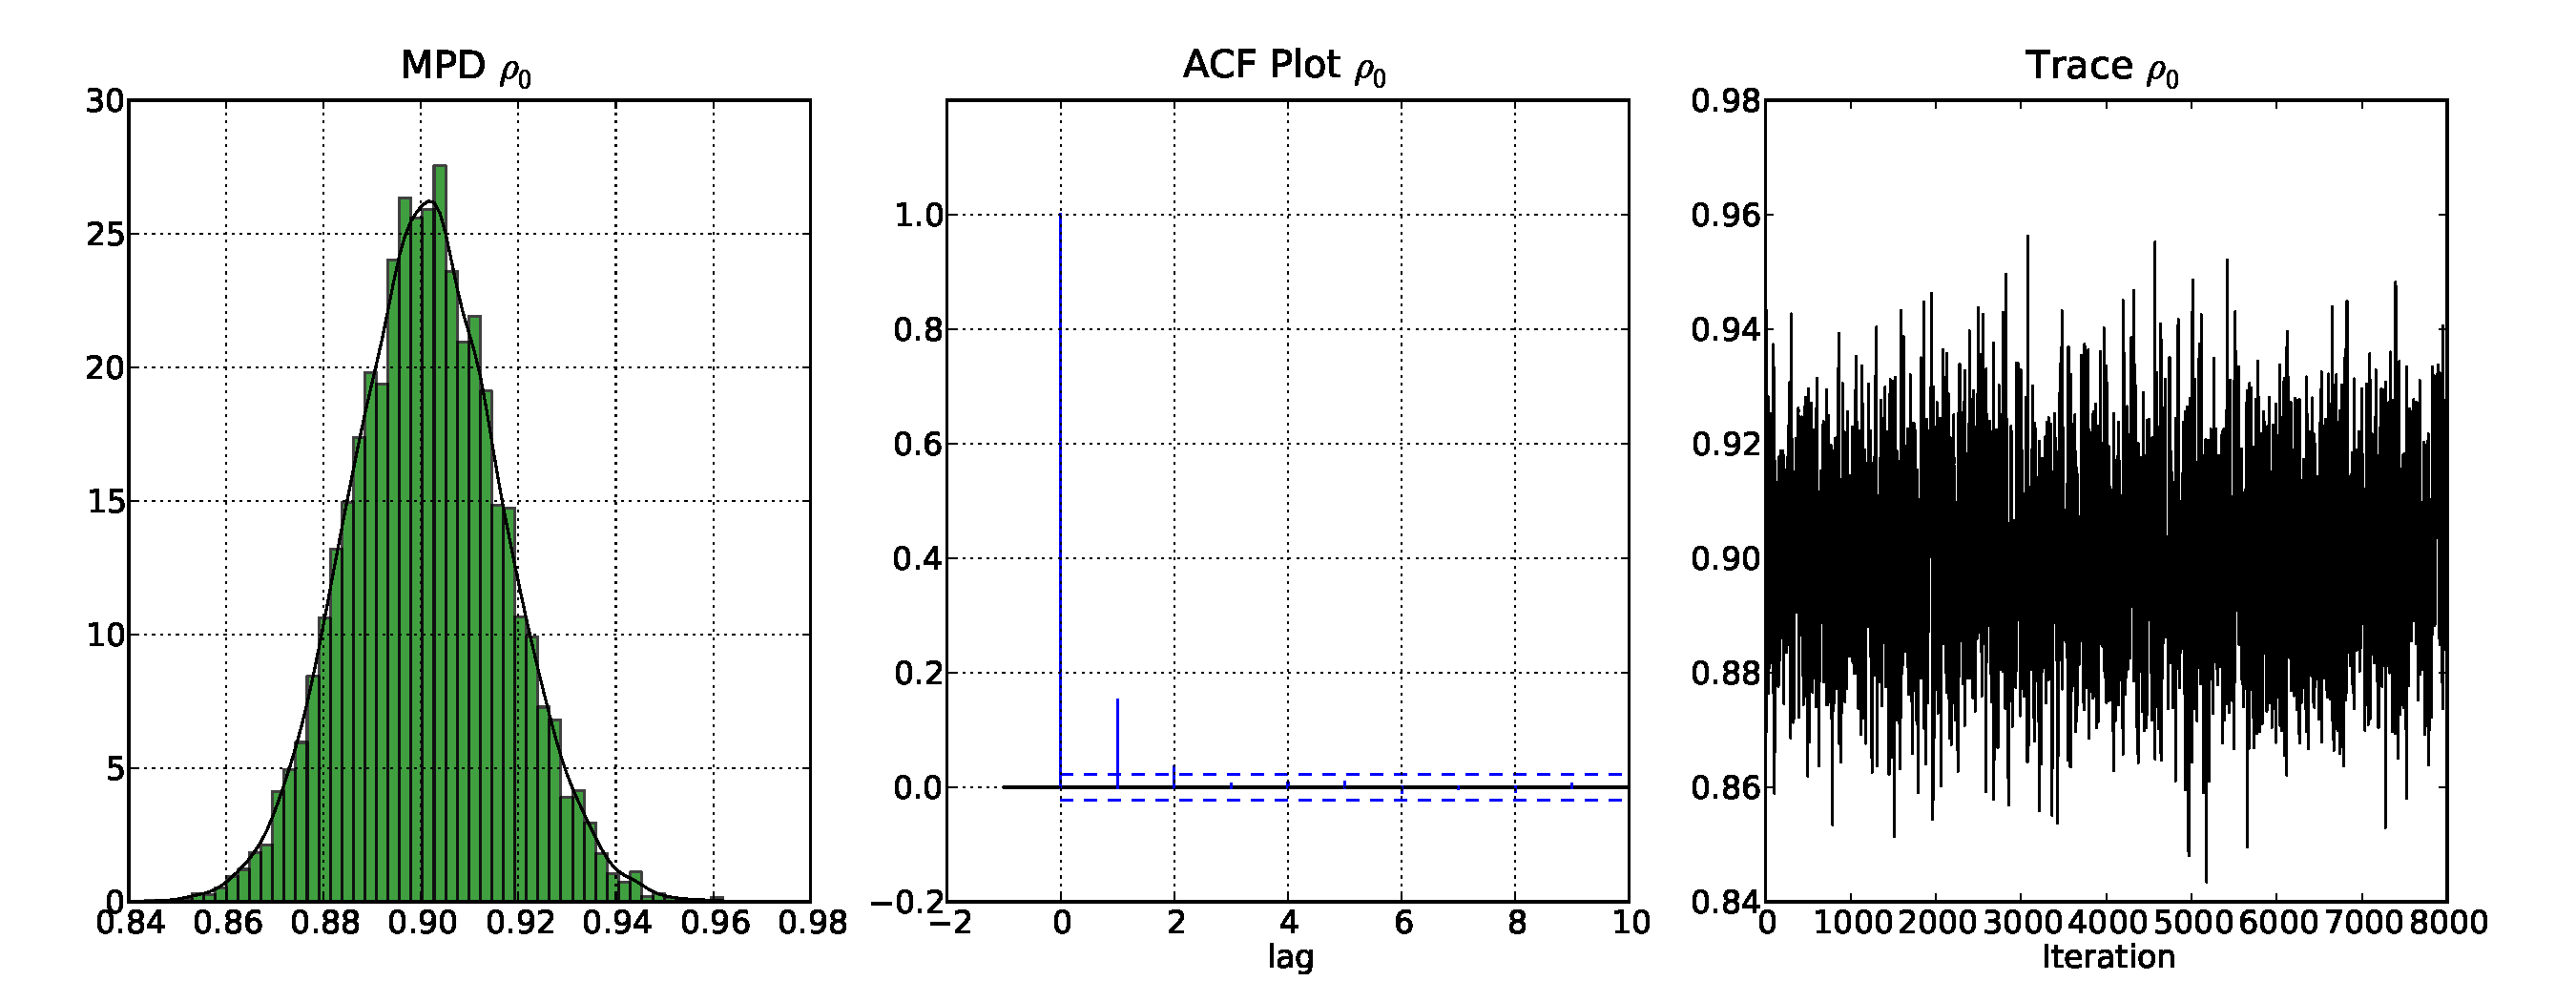
\includegraphics[scale=0.6]{rho001}\label{Flo:AR1}

\caption{}

\end{figure}


Figure \ref{Flo:AR1} plots the marginal posterior density, autocorrelation
plot and the trace plot for the iterates. 


\section{Using PyMCMC efficiently}

The fact that MCMC algorithms rely on a large number of iterations
to achieve reasonable results and are often implemented on very large
problems, dictates that the user must have the required machinery
to implement efficient code. In MCMC analysis efficiency comes through
an understanding of what makes a simulation efficient MCMC sampler
and also the ability to produce compuationally efficient code. Interestingly
the two are related. To achieve simulation efficient code in MCMC
samplers it is often extremely important that large numbers of parameters
are blocked together. A classic example in the litererature are using
\emph{simulation smoothers }to jointly sample the state vector in
a state space model; see for example Carter and Kohn (1994) and de
Jong and Shephard (1995). Whilst implementing a simulation smoother
is required to achieve simulation efficient code, the sequential nature
of their implementaion often renders higher level languages impractical
for large problems and thus forces the analyst to write their entire
code in lower level languages. This is an innefficient use of time
as usually only small precentage of code needs to be optimised. This
drawback is easily circumvented in PyMCMC as Python makes it so easy
to use a lower level language to write the specialised module and
use the function directly from Python. This ensures PyMCMC's modules
can be used for rapid development from Python and lower level languages
are only resorted to when necessary. This Section aims to provide
guidelines for producing efficient code with PyMCMC. We discuss alternative
external libraries that are available to the user for producing efficient
code using PyMCMC. Despite the ease of writing specialised modules
this however should not be the first resort of the user. Instead one
should ensure that the Python prototypes are efficiently coded using
the resorces available with Python.

Arguably, the first thing the user of PyMCMC should concerntrate on
when optimising there PyMCMC code is to ensure they use as many inbuilt
functions and libraries as possible. As most high performance libraries
are written in C or Fortran this ensures that computationally expensive
procedures are computed using code from compiled languages. Python
users, and hence PyMCMC users have an enormous resource of Scientific
libraries available to them as a result of the popularity of Python
in the scientific community. Two of the most important libraries for
most users, will quite possibly be, Numpy and Scipy. Making use of
such libraries is one of the best ways of avoiding large loops in
procedures that are called from the Gibbs sampler. If a large loop
is used inside a function that is called from inside the Gibbs sampler
then this could mean a large proportion of the total computation is
being done by Python, rather than a library that was generated from
optimised compiled code. This can have a dramatic effect on the total
computation time. As a simple and somewhat trivial example we modify
Example \ref{sub:Example-2:-Log-linear} so that a loop is explicitly
used to calculate the log likelihood.


\begin{lstlisting}[basicstyle={\scriptsize}]
def logl(store):
    """function evaluates the log - likelihood for the log - linear model"""
    suml=0.0
    for i in xrange(store['yvec'].shape[0]):
        xbeta=dot(store['xmat'][i,:],store['beta'])
        suml=suml+store['yvec'][i] * xbeta - exp(xbeta)
    return suml
\end{lstlisting}


Whilst the two functions to calculate the log-likelihood are mathematically
equivalent, the one with the explicit loop is substantially slower.
Specifically, the time taken for the Gibbs sampler went from 7.3 seconds
to 130.19 seconds. As such, this minor modification leads to an approximately
18 times decrease in the speed of the program.

If the use of an an inbuilt function is not possible and the time
taken from the program is unexceptable then there are several alternative
solutions available to the user. One such solution is to use the package
Weave, which is a part of Scipy, to write inline C code to accelerate
the problem area in the code. An example is given below.


\begin{lstlisting}[basicstyle={\scriptsize}]
def logl(store):
    """function evaluates the log - likelihood for the log - linear model"""

    code = """     
		double sum = 0.0, xbeta;
		for(int i=0; i<nobs; i++){
			xbeta = 0.0;
			for(int j=0; j<kreg; j++){xbeta += xmat[i+j*kreg] * beta[j];}
			sum += yvec[i] * xbeta - exp(xbeta);
		}     
		return_val = sum;
    """
    yvec = store['yvec']
    xmat = store['xmat']
	nobs, kreg = xmat.shape
	beta = store['beta']
    return weave.inline(code,['yvec','xmat', 'beta','nobs','kreg'],\ 
                       compiler='gcc')
\end{lstlisting}


The total time taken for weave version is 4.33 seconds. The reason
for the speed increase over the original version that uses numpy functions
is the weave version avoids the construction of temporary matricies
that are typically a by product of overloaded operators. 

Another alternative, which is our prefered approach, is to use F2py,
which allows for the seamless integration of Fortran and Python code.
Following on with the same trivial example we use the following Fortran77
code. The examples requires that the user the have basic linear algebra
subprograms (BLAS) and and preferable also the automatically tuned
linear algebra software (ATLAS).\\
 
\begin{lstlisting}[basicstyle={\scriptsize}]
c     fortran 77 code used to calculate the likelihood of a log
c     linear model. Subroutine uses BLAS.

      subroutine logl(xb,xm,bv,yv,llike,n,k)
      implicit none
      integer n, k, i, j
      real*8 xb(n),xm(n,k), bv(k), yv(n), llike
      real*8 alpha, beta

cf2py intent(in,out) logl
cf2py intent(in) yv
cf2py intent(ini bv
cf2py intent(in) xmat 
cf2py intent(in) xb 

      alpha=1.0
      beta=0.0
      call dgemv('n',n,k,alpha,xm,n,bv,1,beta,xb,1)

      llike=0.0
      do i=1,n
          llike=llike+yv(i)*xb(i)-exp(xb(i))
      enddo
      end
\end{lstlisting}


The code is compiled with the command:

f2py -c loglinear.f -m loglinear -lblas -latlas

then called from Python as follows


\begin{lstlisting}
import loglinear
\end{lstlisting}


The loglinear library must be imported to be accessible and is done
as above. The log-likelihood function is then modified as follows


\begin{lstlisting}[basicstyle={\scriptsize},numbers=left]
def logl(store):
	"""function evaluates the log - likelihood for the log - linear model"""
	loglike=array(0.0)     
	return loglinear.logl(store['xb'],store['xmatf'], store['beta'],store['yvec'],loglike)
    
\end{lstlisting}


The code is further in example1c.py is further modified by inserting
the following code before line 59 in the original program.


\begin{lstlisting}
data['xb']=zeros(yvec.shape[0])
data['xmatf']=asfortranarray(xmat)
\end{lstlisting}


The array \emph{data{[}'xb'{]}} is simply a work array used for the
calculation of $\bm{X}\bm{\beta}.$ It is stored in in the Python
dictionary data, simply so it is only created once rather that each
time the function \emph{logl} is called. The second array \emph{data{[}'xmatf'{]}}
simply stores $\bm{X}$ in column major order, which is what is used
in Fortran, rather than the Python default, which is row major order
the default for the C programming language. If \emph{store{[}'xmat'{]}}
is passed to the function \emph{loglinear.logl} then f2py will automatically
produce a copy and convert it to column major order each time the
function \emph{logl} is called.

The total time for the Gibbs sampler when using f2py is 4.03 seconds.
This is slightly faster that the version that uses Weave, where most
likely the small gain can be attributed to the use of ATLAS.

The user has many other choices available to them for writing specialised
extension modules. For example, if it is the preference of the user
it is not much more difficult to use F2py to compile procedures written
in C, which then can be used directly from Python. Another popular
library that can be used to marry C, as well as C++, code with Python
is SWIG. In our opinion Swig is more difficult than f2py for complicated
examples. The user may also opt to manually call C and C++ routines
using Python and Numpy's C application interface. Another option for
C++ users is to use Boost Python. These alternative approaches are
beyond the scope of this paper.


\section{PyMCMC interacting with R}

There are a number of functions from the R statistical language (REF)
that can be useful in Bayesian analysis. These can be accessed in
PyMCMC through the RPy2 python library (REF). In PyMCMC, we show how
this can be approached prior to the Bayesian analysis, and also to
explore and summarise the MCMC output. As an example, consider the
Log linear model described in Section\textasciitilde{}\textbackslash{}ref\{sub:Example-2:-Log-linear\}.
The random walk MH requires the specification of a candidate density
function (Equation\textasciitilde{}\ref{eq:log_lin_candidate_dist})
and an initial value. The R functions \texttt{glm }and \texttt{summary.glm}
can be used to set this to the maximum likelihood estimate$\hat{\beta}$and
the unscaled estimated covariance matrix of the estimated coefficients.
The relevant code is summarised below:


\begin{lstlisting}[basicstyle={\scriptsize},numbers=left,tabsize=4]
import rpy2.robjects.numpy2ri
from rpy2 import rinterface
import rpy2.robjects as robjects
...
def initial_values(yvec,xmat):
    '''
    Use rpy2 to get the initial values
    '''
    ry = rinterface.SexpVector(yvec,rinterface.INTSXP)
    rx = rinterface.SexpVector(xmat[:,1:],rinterface.INTSXP)
    robjects.globalenv['y'] = ry
    robjects.globalenv['x'] = rx
    mod = robjects.r.glm("y~x", family="poisson")
    init_beta =  array(robjects.r.coefficients(mod))
    modsummary = robjects.r.summary(mod)
    scale = array(modsummary.rx2('cov.unscaled'))
    return init_beta,scale

#main program
random.seed(12345)       #seed or the random number generator

data=loadtxt('count.txt',skiprows=1)    #loads data from file
yvec=data[:,0]
xmat=data[:,1:data.shape[1]]
xmat=hstack([ones((data.shape[0],1)),xmat])

data={'yvec':yvec,'xmat':xmat} 

#use R to obtain the initial vector for beta and the scale matrix
init_beta,scale=initial_values(yvec,xmat)

samplebeta=RWMH(posterior,scale,init_beta,'beta')
GS=Gibbs(20000,4000,data, [samplebeta],loglike=(logl,xmat.shape[1],'yvec'))
GS.sampler()
GS.CODAoutput(filename="loglinear_eg") 

\end{lstlisting}


It may also be useful to take advantage of the many MCMC analysis
functions in R and associated packages. To facilitate this, PyMCMC
includes a CODA ref(XXX) output format which can easily be read into
R for further analysis. A sample R session after PyMCMC might look
like:


\begin{lstlisting}[basicstyle={\scriptsize},language=R,numbers=left]
library(coda)
aa <- read.coda("loglinear_eg.txt","loglinear_eg.ind")
plot(aa)
summary(aa)
raftery.diag(aa)
xyplot(aa)
densityplot(aa)
acfplot(aa,lag.max=500)

\end{lstlisting}



\section{Conclusions}

In this paper, we have described the Python software package PyMCMC.
PyMCMC takes advantage of the flexibility and extensibility of Python
to provide the user with a code efficient way of constructing MCMC
samplers. The PyMCMC package includes classes for Gibbs sampler the
MH, independent MH, random walk MH, OBMC and slice sampling algorithms.
It also contains and inbuilt module for Bayesian regression analysis.
We demonstrate PyMCMC using an example of Bayesian regression analysis
with stochastic variable selection, a log-linear model and also a
time series regression analysis with first order autoregressive errors.
We demonstrate how to optimise PyMCMC using Numpy functions, inline
C code using Weave and with Fortran77 using F2py, where necessary.
We further demonstrate how to call R functions using R2py. 


\subsection*{Acknowledgements}

This research has been supported by an Australian Research Council
Linkage Grant; ???????? 

\bibliographystyle{plain} \bibliographystyle{plain}
\bibliography{/home/chris/Dropbox/Projects/Bibtex/chris}

\end{document}
